%\documentclass[a4paper, 12pt]{report}
\documentclass[12pt,a4paper,openany]{abntex2}

\usepackage[T1]{fontenc}
%\usepackage[latin1]{inputenc}
%\usepackage[verbose,left=30mm,right=20mm,top=30mm,bottom=30mm]{geometry}
%\usepackage{txfonts}
\usepackage[brazil]{babel}
\usepackage{pdfpages}
%\usepackage[authoryear]{natbib}
%\usepackage{appendix}
%\usepackage{setspace}
%\usepackage{url}
%\usepackage{hyperref}
%\usepackage{color}
\usepackage[utf8]{inputenc}
\usepackage{placeins}
\usepackage{float}

\autor{Leonardo Mendonça de Araujo \and \\ Lucas Bagatini do Nascimento \and \\ Mário Muramatsu Júnior}
\titulo{RELATÓRIO DE FINAL: IDENTIFICADOR DE SINAIS TRIFÁSICOS}
\data{2018} 
\local{Rio Claro, São Paulo}
\preambulo{Monografia apresentada ao curso de Ciências da Computação, como requisito parcial para a obtenção do Título de Bacharel em Ciências da Computação, Instituto de Geociências e Ciências Exatas da Universidade Estadual Paulista}
\orientador{Mario Roberto da Silva}
\tipotrabalho{monografia}

\begin{document}
	
\imprimircapa	
\imprimirfolhaderosto

\clearpage
\cleardoublepage
\cleardoublepage

\pagenumbering{arabic}
\setcounter{page}{3}

\tableofcontents
\clearpage{\pagestyle{empty}\cleardoublepage}
	
\chapter{Introdução}

\section{Sistemas Elétricos Polifásicos}

Naturalmente, sistemas elétricos funcionando em corrente alternada possuem picos e vales de tensão e, consequentemente, picos e vales de potência. A fim de mitigar esta ineficiência intrínseca, pode-se montar um sistema polifásico, ou seja, um sistema que fornece energia elétrica através de três ou mais condutores energizados.

As figuras ~\ref{fig:sinal-bifasico} e ~\ref{fig:sinal-trifasico} ilustram o comportamente da tensão em sistemas bifásicos e trifásicos, respectivamente. É trivial perceber que sistemas polifásicos são capazes de fornecer tensão de maneira mais constante e sem necessitar de altos picos em cada uma de suas fases.
 
\begin{figure}[!htp]
	\centering
	\fbox{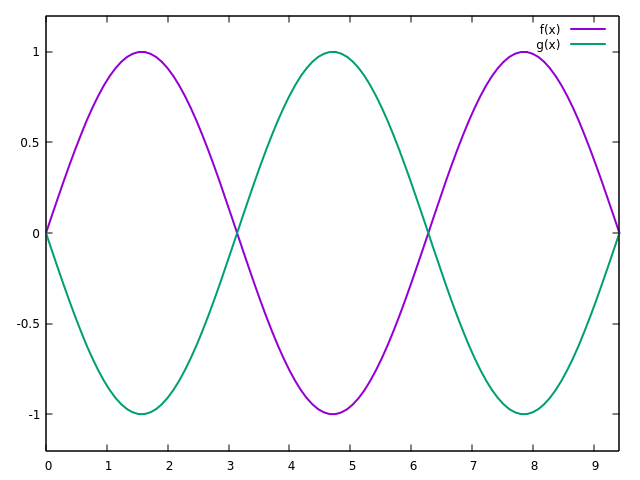
\includegraphics[width=16cm]{./images/Bifasico.png}}
		\caption{Exemplo de sistema Bifásico}
	\label{fig:sinal-bifasico}
\end{figure}

\begin{figure}[!htp]
	\centering
	\fbox{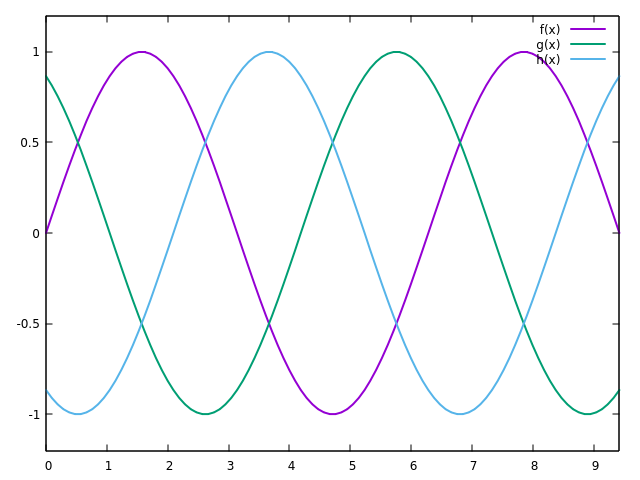
\includegraphics[width=16cm]{./images/Trifasico.png}}
		\caption{Exemplo de sistema Trifásico}
	\label{fig:sinal-trifasico}
\end{figure}


\section{Sistemas Trifásico: Usos e Vantagens}

Como discutido acima, um sistema trifásico de transmissão (que se utiliza de três condutores) de energia possui diversas vantagens sobre sistemas monofásicos (que usam dois condutores). Dentre eles, o mais notório é o ganho em custo-benefício de tal sistema. Pode-se transmitir o triplo da energia com somente 50\% de incremento nos custos.

Sistemas polifásicos são especialmente úteis e convenientes na construção e operação de motores elétricos, tal qual os motores de indução, por serem capazes de produzirem campos magnéticos rotativos de intensidades mais constantes e confiáveis. É possível alterar a frequência das três fases para alterar a velociade de rotação do motor, por exemplo. Motores de indução que utilizam corrente contínua requerem diversas peças adicionais, como transformadores, que encarecem o mecanismo final.

De maneira análoga à motores de indução, sistemas de distribuição trifásicos são capazes de aproveitar mais da energia gerada por um gerador, como turbinas de uma hidrelétrica.

\section{Projeto: Identificador de Sinais Trifásicos}

Ao longo de grandes instalações elétricas, ao se utilizar modelos trifásicos, deve-se garantir que os diversos dispositivos e conexões estão ligados às fases adequadas. Erros desta natureza podem causar desde ineficiência do maquinário ligado até catastróficos acidentes. A fim de auxiliar na tarefa, propõe-se que seja construído um Identificador de Fase para Sinais Trifásicos.

Sabendo-se que duas linhas fazem parte de sistemas de transmissão trifásicos, o aparato deve ser capaz de fazer a leitura da frequência de um e compará-la à frequência do outro, indicando se há ou não defasagem entre ambas. Deve-se construir também um sistema que garanta a confiabilidade da leitura, 


%----------------Exemplo: insere figura-----------------------
%\begin{figure}[!htp]
%	\centering
%	\fbox{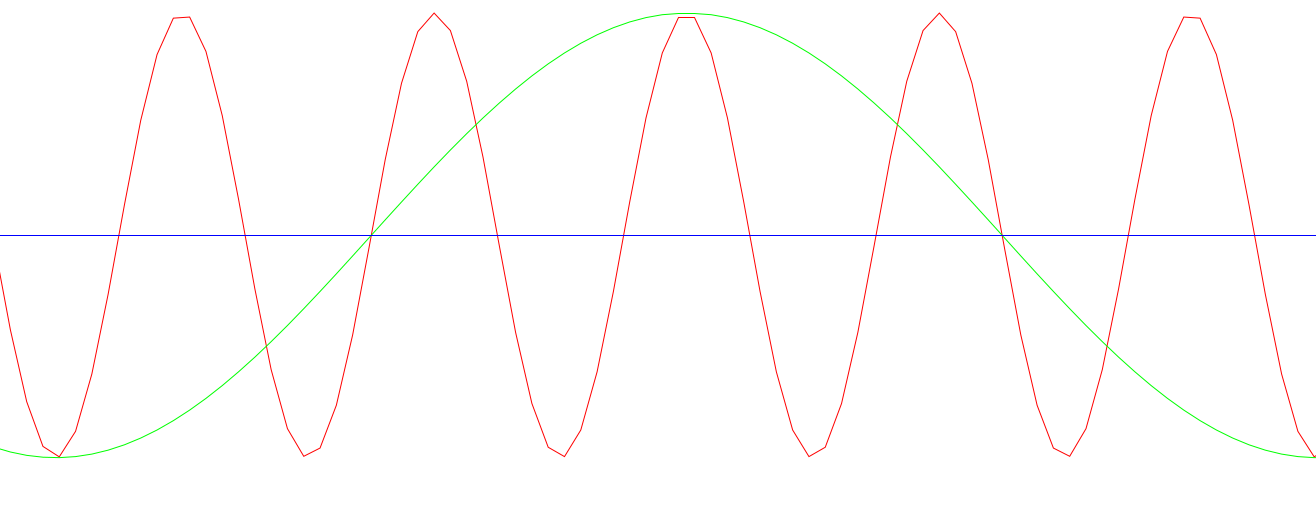
\includegraphics[width=16cm]{images/ondas.png}}
%		\caption{Exemplo de ondas sonoras}
%	\label{fig:ondas-sonoras}
%\end{figure}


%---------------Exemplo: insere tabela -----------------------
%\begin{table}[h]	
%	\centering	
%	\vspace{0.5cm}	
%\begin{tabular}{r|lr}
%Notas  & Frequ{\^e}ncia (Hz) \\
%\hline 
%C (Dó) & 261,33          \\
%D (Ré) & 293,66          \\
%E (Mi)  & 329,63 		 \\
%F (Fá)  & 349,23 		 \\
%G (Sol) & 391,99 		 \\  
%A (Lá)  & 440,00  		 \\
%B (Si)  & 493,88
%\end{tabular}
%	\label{tab:frequencia-notas}
%	\caption{Frequência da notas centrais do piano}
%\end{table}

\end{document}
